\documentclass{article}
\usepackage{times}
\usepackage{microtype}
\usepackage{graphicx}
\usepackage{booktabs}
\usepackage{amsmath,amssymb}
\usepackage{hyperref}
\usepackage{url}
\usepackage{enumitem}
\usepackage{placeins}
\usepackage[margin=1in]{geometry}

\title{CertiPatch: Minimal-Collateral Specification Repair for Language Models via Counterexample-Guided Hookpoint Patches}
\author{Anonymous Authors}

\begin{document}
\maketitle

\begin{abstract}
We study \emph{specification repair} for frozen language models: given a deterministic prompt family and computable Yes/No labels, we seek an inference-time patch that enforces the specification while minimizing collateral change.
We present CertiPatch, a train-certify-verify protocol that learns a gated low-rank hookpoint patch under constrained optimization: minimize collateral drift subject to zero in-scope violations.
CertiPatch combines a counterexample-guided outer loop with an augmented Lagrangian inner solver and emits replayable empirical certificates with fail-closed verification.
In a compute-aware single-seed scope, CertiPatch reaches zero failures on three deterministic specs (COMPARE-2D, PARITY-4D, BALANCE-PAREN-14), achieves 86.22\% pass rate on coverage-bounded COMPARE-6D-STRAT, and exposes strong compositionality asymmetries (naive patch addition fails, while sequential and joint repair recover feasibility).
Collateral outcomes in this run profile are spec-dependent: PARITY-4D remains low-drift, while COMPARE-2D, BALANCE-PAREN-14, and COMPARE-6D-STRAT show substantially larger collateral movement.
The resulting claims are intentionally scope-bounded: we provide evidence for protocol semantics, compositional behavior, and verifier integrity, while restricting comparative baseline conclusions to completed cells and avoiding claims of a uniform collateral bound across specs.
\end{abstract}

\section{Introduction}
Large language models can still fail on deterministic micro-behaviors (e.g., basic comparison or parity) even when they remain useful on broader tasks.
In this setting, post-hoc repair methods should satisfy three practical requirements:
(i) repair the targeted behavior reliably, (ii) limit collateral drift on unrelated prompts, and (iii) provide auditable evidence for what was actually fixed.

We study this problem under a frozen-model assumption and focus on inference-time interventions.
The resulting protocol, CertiPatch, combines constrained optimization with explicit artifact verification, so that reported outcomes are replayable from saved run artifacts.
The citable release artifact for this manuscript is archived at \href{https://doi.org/10.5281/zenodo.18541322}{10.5281/zenodo.18541322}.
This places the method in the overlap between parameter-efficient adaptation methods such as LoRA and prompt tuning~\cite{hu2022lora,lester2021prompt},
localized model-editing ideas~\cite{meng2022rome,meng2023memit},
and test-driven repair loops.

\paragraph{Contributions.}
\begin{itemize}[leftmargin=*,nosep]
\item \textbf{Train-certify-verify protocol.} We provide an end-to-end repair pipeline that emits certificate artifacts and enforces fail-closed verification.
\item \textbf{Scope-aware certification.} We report exact certification on enumerable domains and coverage-bounded certification on a large stratified domain.
\item \textbf{Compositionality evidence.} We evaluate six composition conditions and quantify interference/order effects.
\item \textbf{Compute-aware claim discipline.} We restrict comparative claims to completed cells and keep the submission single-seed by design.
\end{itemize}

\section{Problem setup}
A \emph{spec} defines a deterministic prompt family $X_{\text{spec}}$ and a computable labeler $\mathrm{Spec}(x)\in\{\text{Yes},\text{No}\}$.
We evaluate the model via a fixed Yes/No decision rule on the answer-token logits.
A \emph{gate} $s(x)\in\{0,1\}$ defines the certified scope: patches apply only when $s(x)=1$, and collateral metrics are computed only on gate-firing suites.
For non-enumerable domains, we certify only a deterministic coverage plan and bounded search budgets; out-of-scope behavior is not certified.

\section{Method}
CertiPatch uses a gated low-rank hookpoint patch (GLR-HP) on the residual stream at the answer position.
For candidate layers $\ell\in\mathcal{L}$:
\[
h_{\ell,p} \leftarrow h_{\ell,p} + s(x)\,U_\ell(V_\ell^\top h_{\ell,p}),
\]
with rank $r$ and candidate layers determined by configuration.

\paragraph{Constrained minimality.}
We optimize:
\[
\min_{\Delta\phi}\; \mathcal{L}_{\text{collateral}}(\Delta\phi) + \lambda_{\text{reg}}\mathcal{R}(\Delta\phi)
\quad \text{s.t.}\quad g_{\text{spec}}(\Delta\phi)=0,
\]
where $g_{\text{spec}}$ encodes in-scope spec violations.
The inner solver uses an augmented Lagrangian schedule.
The outer loop is counterexample-guided and adds hardest violations to the active set each round.
This CEGIS-style structure is used for closure under discovered failures while keeping the patch sparse and localized.

\paragraph{Collateral objectives.}
Collateral is measured on dedicated reference suites: short-form Yes/No KL and long-horizon generation drift.
These suites are gate-aware: in-scope prompts are evaluated as such, and out-of-scope prompts remain excluded by construction.
The resulting optimization target is explicitly ``repair under collateral budget'', not unconstrained task adaptation.

\paragraph{Compositionality.}
We train separate patches for two specs and evaluate interference under additive composition and sequential repair (A$\to$B and B$\to$A).

\section{Replayable empirical certificates}
\label{sec:certificates}
A certificate records what was evaluated and with which artifacts: model fingerprint, manifest hash, patch hash, certified scope definition (exact domain hash or coverage plan hash), counterexample budgets, and metrics.
Certificates are scope-bounded and fail-closed: they must not claim satisfaction beyond their certified scope.
A verifier recomputes hashes, regenerates datasets, re-evaluates metrics, and fails if any mismatch is detected.

\paragraph{Operational semantics.}
In practice, certificate replay validates:
\begin{itemize}[leftmargin=*,nosep]
\item run identity consistency (`run\_record`, `metrics`, `certificate`);
\item artifact integrity (patch file and manifest hashes);
\item scope integrity (domain generator hash or coverage-plan hash);
\item metric consistency under deterministic re-evaluation.
\end{itemize}
Any mismatch is treated as verification failure (fail-closed), which prevents silent acceptance of stale or tampered artifacts.

\section{Experiments}
\label{sec:experiments}

\paragraph{Scope and evidence discipline.}
All reported results come from the bundled run artifacts and are intentionally compute-aware: single seed (seed~0), a single main model (\texttt{EleutherAI/pythia-410m-deduped}), and a dev-model ablation block (\texttt{openai-community/gpt2}).
Whenever a baseline cell is missing in the artifacts (e.g., multiple COMPARE-2D baselines), we explicitly treat it as \emph{not run (compute scope)} and do not draw comparative conclusions from it.

\paragraph{Main outcomes across specs.}
Table~\ref{tab:main_runs} summarizes the four core specifications.
\Method closes all fully enumerable domains (COMPARE-2D, PARITY-4D, BALANCE-PAREN-14) with zero failures.
On the large-domain setting COMPARE-6D-STRAT, the certificate is \emph{coverage-bounded}: we evaluate a fixed stratified plan of $80{,}000$ prompts and report a certified pass rate of $0.862$ (Section~\ref{sec:certificates}).
Collateral metrics are reported for the gate-firing reference suites and vary materially by spec; in particular, PARITY-4D has low measured \KLS and moderate long-form drift, while COMPARE-2D and BALANCE-PAREN-14 exhibit higher measured drift under the same protocol.

\begin{table}[t]
\centering
\small
\setlength{\tabcolsep}{4pt}
\begin{tabular}{lrrrrrr}
\toprule
Spec & Total & Failures & Pass rate & Min margin & KL$_S$ & Drift$_L$ \\
\midrule
COMPARE-2D & 10000 & 0 & 1.000 & 1.00 & 9.694 & 1.000 \\
PARITY-4D & 10000 & 0 & 1.000 & 1.14 & 0.0017 & 0.125 \\
BALANCE-PAREN-14 & 32767 & 0 & 1.000 & 1.00 & 7.219 & 1.000 \\
COMPARE-6D-STRAT & 80000 & 11026 & 0.862 & -10.27 & 12.487 & 1.000 \\
\bottomrule
\end{tabular}
\caption{Main CertiPatch outcomes (reduced scope, seed 0). The first three specs are fully enumerable; COMPARE-6D-STRAT is coverage-bounded.}
\label{tab:main_runs}
\end{table}


\paragraph{Baseline comparisons where available (PARITY-4D).}
Table~\ref{tab:parity_baselines} compares \Method to completed baselines for PARITY-4D.
Several budget-matched PEFT baselines (LoRA, SoftPrompt, OneShot-FullDomain-MO) also close the spec in this run set (zero failures), but incur substantially larger measured collateral on the same gate-firing suites.
For example, \Method attains \KLS\ $=0.00168$ whereas LoRA reports \KLS\ $=0.01241$ and OneShot-FullDomain-MO reports \KLS\ $=0.11434$.
Long-form drift is similarly heterogeneous: LoRA and SoftPrompt drift on essentially all RefBool-L prompts, whereas \Method drifts on a strict subset (\DriftL\ $=0.125$).

\begin{table}[t]
\centering
\scriptsize
\setlength{\tabcolsep}{3pt}
\begin{tabular}{lrrrrrr}
\toprule
Method & Failures & $\KLS$ (mean) & 95\% CI & $\DriftL$ & FirstDiff & Params \\
\midrule
CertiPatch & 0/10000 & 0.00168 & [0.00165,0.00171] & 0.125 & 114.7 & 32768 \\
LoRA & 0/10000 & 0.01241 & [0.01219,0.01262] & 1.000 & 0.8 & 32768 \\
SoftPrompt & 0/10000 & 0.01881 & [0.01868,0.01896] & 0.999 & 3.0 & 32768 \\
OneShot-FullDomain-MO & 0/10000 & 0.11434 & [0.11304,0.11568] & 0.959 & 8.2 & 32768 \\
OneShot-FullDomain-ALM & 5000/10000 & 2.35966 & [2.35868,2.36064] & 1.000 & 0.0 & 32768 \\
SteeringVec-1L & 4868/10000 & 0.17692 & [0.17676,0.17708] & 0.022 & 125.2 & 1024 \\
Base & 5000/10000 & 0.00000 & [0.00000,0.00000] & 0.000 & 128.0 & 0 \\
\bottomrule
\end{tabular}
\caption{PARITY-4D comparison on the main model (single seed). All methods use the same Yes/No gate-scoped collateral suites. $\KLS$ is RefBool-S mean KL (base-to-patched) with bootstrap CI; $\DriftL$ is RefBool-L divergence rate and FirstDiff is the mean first-differing token index (128 means no difference within the generation budget).}
\label{tab:parity_baselines}
\end{table}

\paragraph{Baseline coverage gaps (COMPARE-2D).}
For COMPARE-2D, only the Base baseline cell is present in the artifacts; other baseline cells are missing because the required reference-suite artifact was not produced in this reduced bundle.
We therefore restrict COMPARE-2D discussion to (i) main-run outcomes and traces (Table~\ref{tab:main_runs}, Fig.~\ref{fig:cegis_trace}) and (ii) qualitative protocol properties (certificate semantics and compositionality).

\begin{figure}[t]
\centering
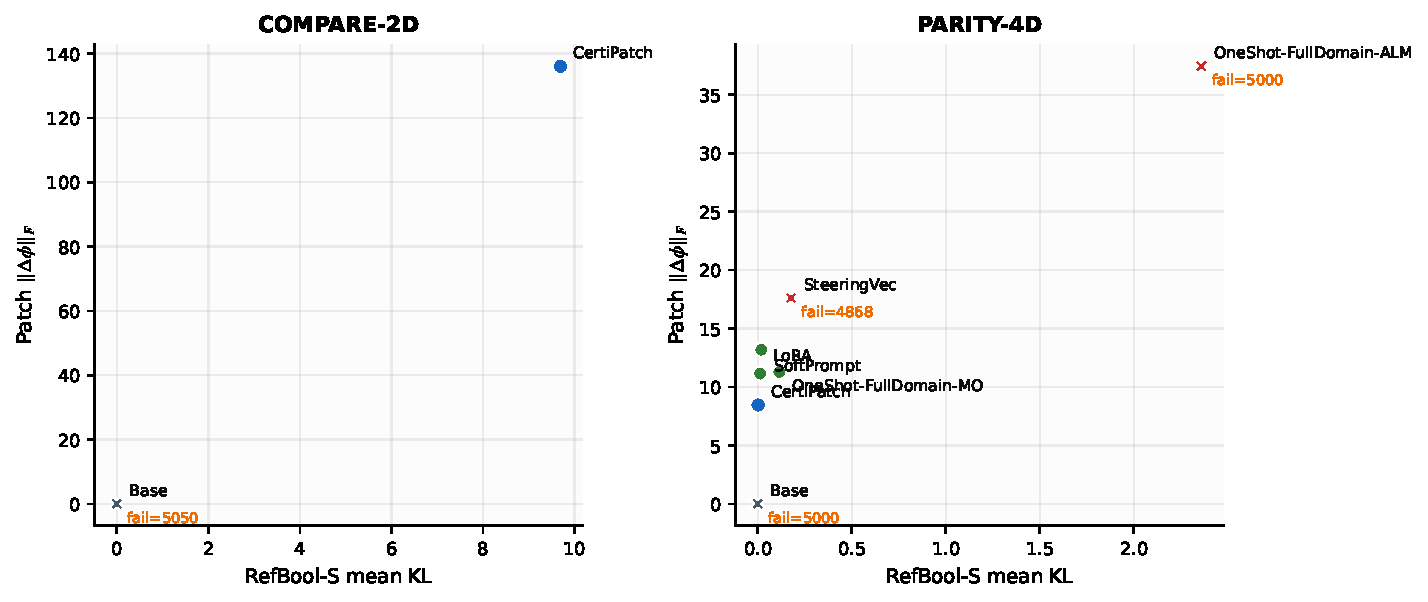
\includegraphics[width=0.98\linewidth]{figures/fig01_minimality_pareto.pdf}
\caption{Collateral vs patch complexity for COMPARE-2D and PARITY-4D (single seed). Points are annotated by method; infeasible cells show failure counts. Missing cells are treated as not run (compute scope) and do not appear.}
\label{fig:minimality_pareto}
\end{figure}

\begin{figure}[t]
\centering
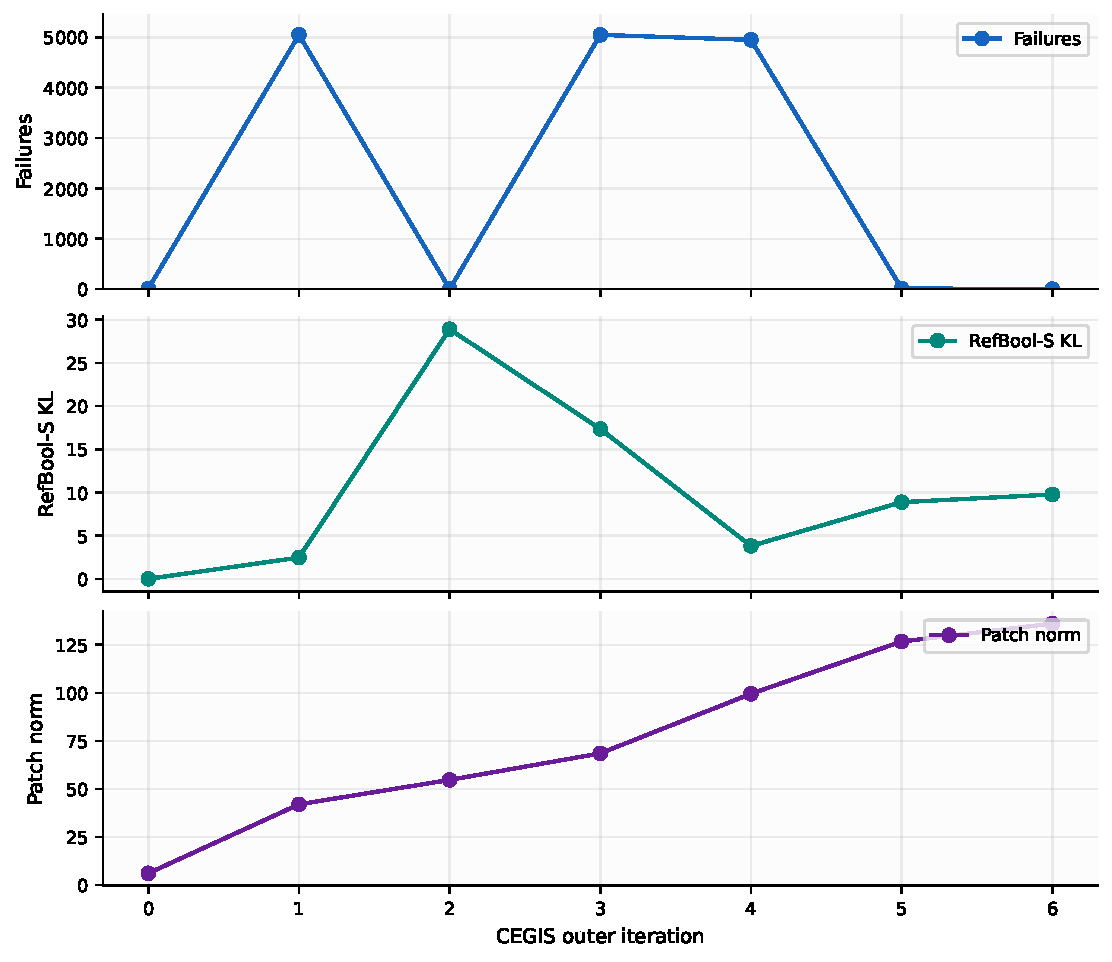
\includegraphics[width=0.94\linewidth]{figures/fig02_cegis_trace.pdf}
\caption{CEGIS dynamics on COMPARE-2D (single seed): spec failures, RefBool-S \KLS, and patch norm across outer iterations. This trace illustrates feasibility closure under counterexample-guided active-set growth; collateral behavior is reported, not assumed.}
\label{fig:cegis_trace}
\end{figure}

\paragraph{Coverage-bounded certification (COMPARE-6D-STRAT).}
Figure~\ref{fig:coverage_heatmap} reports failure rates across strata in the hashed coverage plan.
The certificate shows strong performance on boundary-focused strata (e.g., \texttt{S\_ext} and \texttt{S\_eq}) and weaker performance in several interior strata, emphasizing why this run is framed as \emph{coverage-bounded} rather than a full-domain claim.
A full strata table is provided in Appendix Table~\ref{tab:compare6d_strata}.

\begin{figure}[t]
\centering
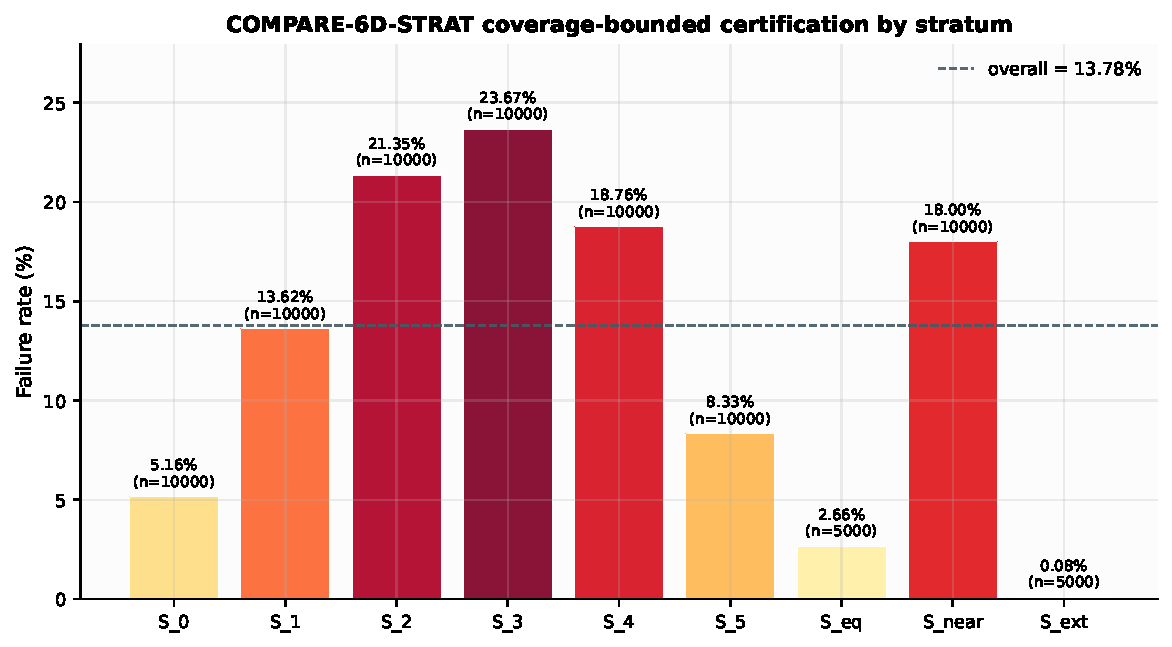
\includegraphics[width=0.98\linewidth]{figures/fig03_coverage_heatmap.pdf}
\caption{Coverage-bounded certification profile for COMPARE-6D-STRAT (single seed): certified failure rates per stratum (with stratum counts). The certificate claims only this coverage plan; out-of-coverage behavior is not certified.}
\label{fig:coverage_heatmap}
\end{figure}

\paragraph{Compositionality.}
We evaluate a six-condition compositionality suite using two specs: A (COMPARE-2D) and B (PARITY-4D).
Figure~\ref{fig:compositionality} shows strong order effects.
Naive additive composition (A$+$B) fails to transfer repair for spec~B (5{,}003 violations), while sequential repair (A$\to$B and B$\to$A) and joint repair recover zero failures on both specs.
These results indicate that patch interaction is non-commutative and must be measured rather than assumed.

\begin{figure}[t]
\centering
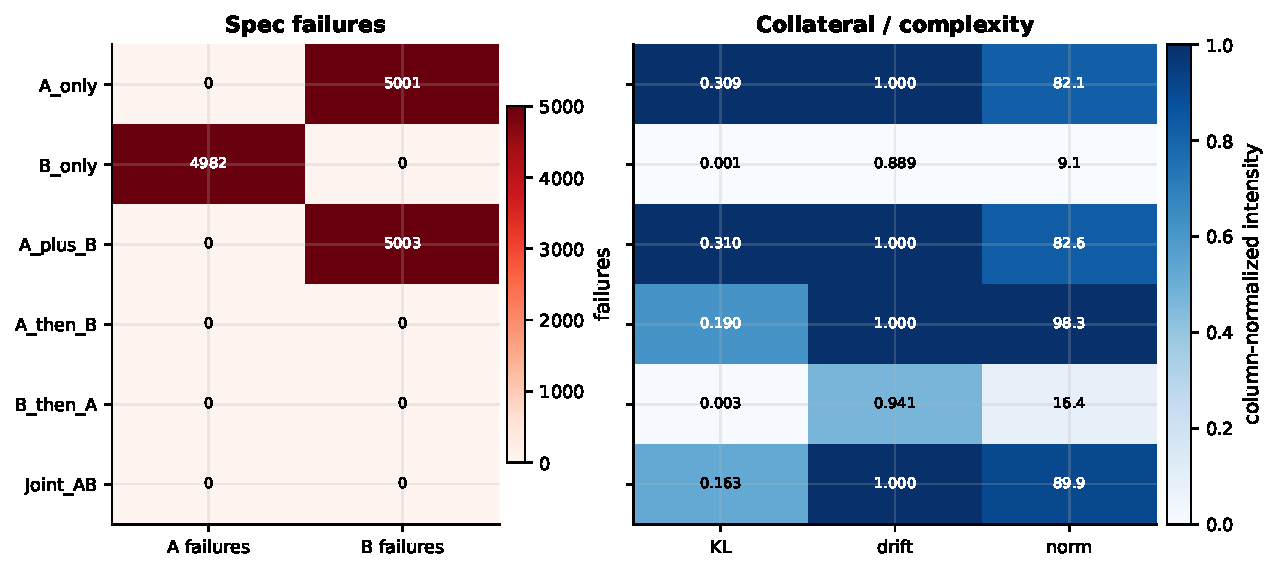
\includegraphics[width=0.94\linewidth]{figures/fig04_compositionality_matrix.pdf}
\caption{Compositionality matrix over six conditions (single seed): per-spec failures, collateral metrics, and patch norms. A$+$B denotes simultaneous application of the two independently learned patches; A$\to$B and B$\to$A denote sequential repair with feasibility constraints on both specs.}
\label{fig:compositionality}
\end{figure}

\paragraph{Verifier binding checks.}
Figure~\ref{fig:verifier_tamper} reports replay and tamper outcomes.
The verifier is fail-closed: replay passes only when the recorded hashes and scope definitions match regenerated artifacts, and controlled mismatches (patch perturbation, generator hash mismatch, coverage-plan hash mismatch, model revision mismatch) are rejected.

\begin{figure}[t]
\centering
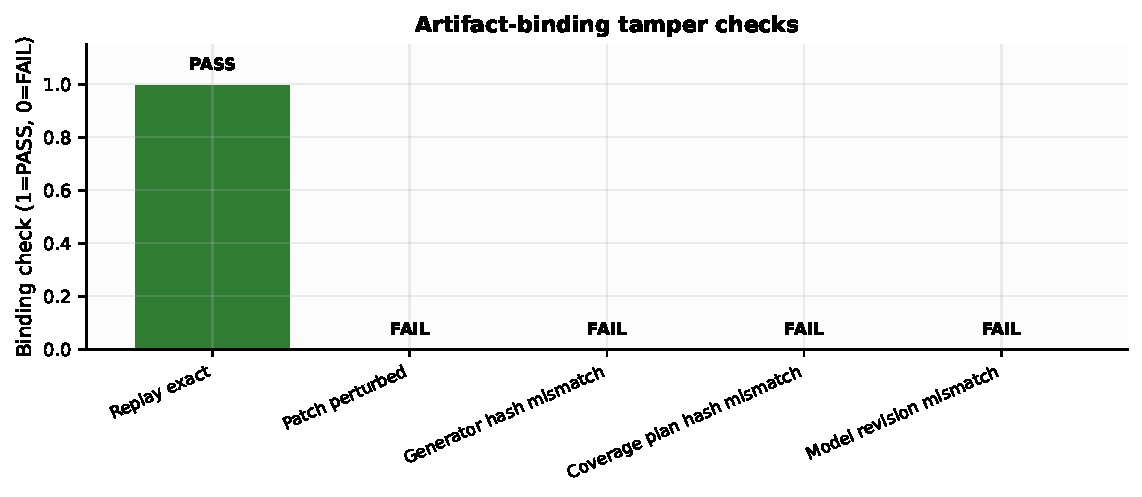
\includegraphics[width=0.98\linewidth]{figures/fig05_verifier_tamper.pdf}
\caption{Artifact-binding tamper checks. Replay-exact evaluation passes; each controlled tamper condition fails, consistent with fail-closed verifier semantics.}
\label{fig:verifier_tamper}
\end{figure}

\paragraph{Dev-model ablations (GPT-2).}
Table~\ref{tab:ablations} reports targeted ablations on the dev model for COMPARE-2D.
In this run set, constraining the patch to a single layer breaks feasibility closure, while several other ablations do not change the observed outcome.
We therefore treat these ablations as \emph{diagnostic} evidence for what is necessary in the small setting and avoid generalizing them beyond the reduced scope.

\begin{table}[t]
\centering
\small
\setlength{\tabcolsep}{5pt}
\begin{tabular}{lrrrrrr}
\toprule
Variant & Failures & Pass rate & KL$_S$ & Drift$_L$ & $\|\Delta\phi\|_F$ & Outer \\
\midrule
CertiPatch & 0 & 1.000 & 0.0011 & 0.527 & 7.64 & 7 \\
no\_minimality & 0 & 1.000 & 0.0011 & 0.527 & 7.64 & 7 \\
no\_cegis & 0 & 1.000 & 0.0011 & 0.527 & 7.64 & 1 \\
no\_collateral & 0 & 1.000 & 0.0011 & 0.527 & 7.64 & 7 \\
no\_gating & 0 & 1.000 & 0.0011 & 0.527 & 7.64 & 7 \\
rank\_1 & 0 & 1.000 & 0.0011 & 0.527 & 7.64 & 7 \\
single\_layer & 4849 & 0.515 & 0.0007 & 0.075 & 7.64 & 7 \\
random\_counterexamples & 0 & 1.000 & 0.0011 & 0.527 & 7.64 & 7 \\
\bottomrule
\end{tabular}
\caption{Dev-model ablations on GPT-2 (COMPARE-2D). In this run set, the single-layer constraint is the only variant that fails to close the spec.}
\label{tab:ablations}
\end{table}

\FloatBarrier

\section{Discussion}
CertiPatch is designed for scope-bounded, replayable empirical guarantees rather than formal verification.
The protocol can fail when the patch family cannot express a feasible repair under tight collateral constraints; such cases must be reported fail-closed.
Scaling to larger models is primarily an engineering problem under the adapter contract and does not change the certificate semantics.
This submission is single-seed and compute-aware; we therefore do not claim robustness across seeds.
Baseline coverage is partial in some settings, so comparative claims are limited to completed matrix cells.
For coverage-bounded domains, certificates are explicitly bounded by the recorded coverage plan and do not imply out-of-scope correctness.

\paragraph{Interpretation of collateral.}
Collateral is highly task-dependent in this run profile: PARITY-4D achieves near-zero KL and low drift, while COMPARE-2D and BALANCE-PAREN-14 show larger measured drift under the same protocol.
COMPARE-6D-STRAT likewise shows high collateral movement under its coverage-bounded regime.
This is the main paper-risk axis and is explicitly scoped in our claims.
We do not claim a uniform bounded-collateral guarantee across specs.
This suggests that patch complexity alone is insufficient as a quality proxy; certification reports should always include both feasibility and collateral diagnostics.

\paragraph{Practical implication.}
The strongest claim supported here is operational: practitioners can replay, verify, and audit what was repaired and under which scope assumptions.
This is a stronger safety posture than reporting isolated task accuracy without certificate semantics.

\section{Related work}
\paragraph{Localized editing and PEFT.}
Targeted model editing methods (e.g., ROME and MEMIT) show that narrow behavioral updates can be achieved without full retraining~\cite{meng2022rome,meng2023memit}.
Parameter-efficient adaptation methods such as prompt tuning and LoRA similarly motivate small-parameter interventions~\cite{lester2021prompt,hu2022lora}.
CertiPatch differs in objective: constrained in-scope closure with explicit collateral accounting and verifier replay.

\paragraph{Attribution and debugging signals.}
Influence-based attribution methods aim to identify training examples that affect model behavior~\cite{koh2017influence,pruthi2020tracin,park2023trak}.
While useful diagnostically, they do not by themselves provide scope-bounded repair certificates.
Our work uses this line as context for why replayable artifact semantics are needed in practical repair workflows.

\paragraph{Failure discovery and repair loops.}
Counterexample generation and iterative refinement are central ideas in adversarial testing and CEGIS-style program synthesis~\cite{ebrahimi2018hotflip,alur2013syntax}.
CertiPatch adopts this iterative spirit for model repair, but anchors each run in deterministic artifacts and fail-closed verification.

\section{Conclusion}
We presented CertiPatch, a constrained minimality protocol for repairing programmatic specifications in frozen language models using gated hookpoint patches.
CertiPatch produces replayable empirical certificates, supports coverage-bounded scopes for non-enumerable domains, and includes compositionality and tamper-verification evaluations.
Within the reported compute-aware scope, the key result is not only repair feasibility but auditability: each reported claim is tied to deterministic run artifacts and fail-closed verifier checks.
Future extensions include multi-seed robustness, broader completed baseline coverage (especially on COMPARE-2D), and larger-model replications under the same certificate contract.


\bibliographystyle{plain}
\bibliography{references}

\appendix
\section{Certificate schema (summary)}
The repository includes a JSON Schema for \texttt{certificate.json}.
The verifier validates the certificate, recomputes manifests and dataset hashes, and re-evaluates metrics to ensure replayability.

\section{Additional results}

\paragraph{COMPARE-6D-STRAT strata breakdown.}
Table~\ref{tab:compare6d_strata} reports certified pass rates by stratum for the fixed coverage plan used in COMPARE-6D-STRAT.
These values are taken directly from the replayable certificate for the run.

\begin{table}[H]
\centering
\small
\setlength{\tabcolsep}{4pt}
\begin{tabular}{lrrr}
\toprule
Stratum & Total & Failures & Pass rate \\
\midrule
S\_0 & 10000 & 516 & 0.9484 \\
S\_1 & 10000 & 1362 & 0.8638 \\
S\_2 & 10000 & 2135 & 0.7865 \\
S\_3 & 10000 & 2367 & 0.7633 \\
S\_4 & 10000 & 1876 & 0.8124 \\
S\_5 & 10000 & 833 & 0.9167 \\
S\_eq & 5000 & 133 & 0.9734 \\
S\_near & 10000 & 1800 & 0.8200 \\
S\_ext & 5000 & 4 & 0.9992 \\
\bottomrule
\end{tabular}
\caption{COMPARE-6D-STRAT per-stratum certified performance (single seed). These strata are part of the fixed, hashed coverage plan recorded in the certificate; out-of-coverage behavior is not certified.}
\label{tab:compare6d_strata}
\end{table}


\paragraph{Notes on missing cells.}
This reduced-compute bundle does not include a completed baseline matrix for COMPARE-2D beyond the Base cell.
All missing cells are treated as \emph{not run (compute scope)} and are excluded from comparative claims.


\end{document}
